\section{Problem statement}
\label{overview:problem}

Software updates pose an important problem. We aim to tackle this problem using
a simple yet effective \emph{multi-version execution} approach: instead of
running only of the software versions, we run multiple versions in parallel; by
carefully coordinating their executions and selecting the behaviour of the more
reliable version when they diverge, we create a more secure and dependable
multi-version application.

\begin{figure}[t]
  \begin{subfigure}[b]{0.5\textwidth}
    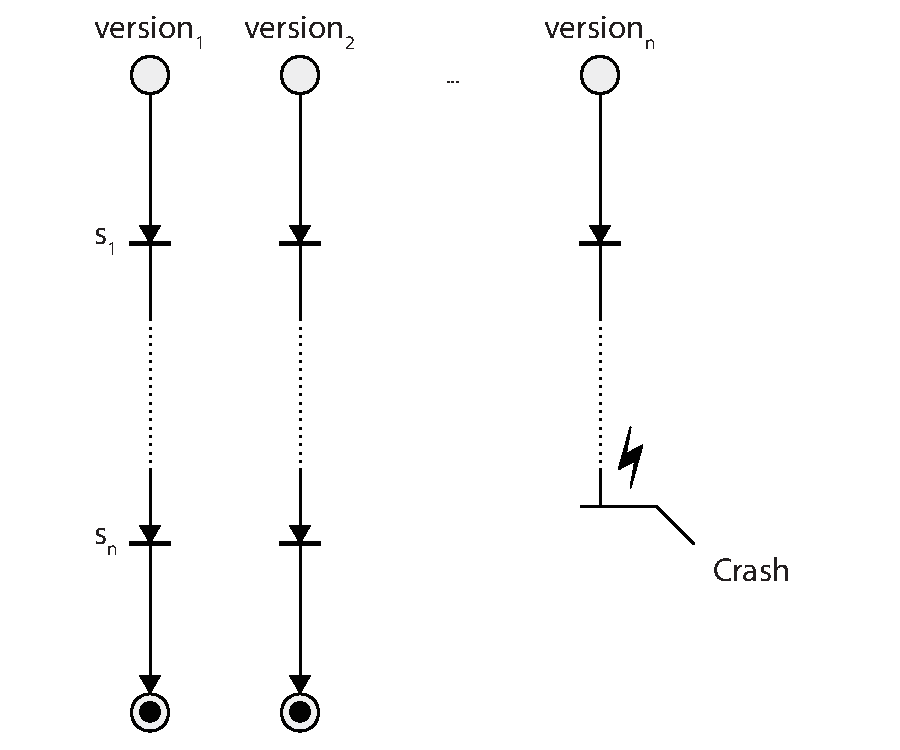
\includegraphics[width=\textwidth]{overview/figures/failover}
    \caption{Failover scheme.}
    \label{fig:failover-scheme}
  \end{subfigure}
  \quad
  \begin{subfigure}[b]{0.5\textwidth}
    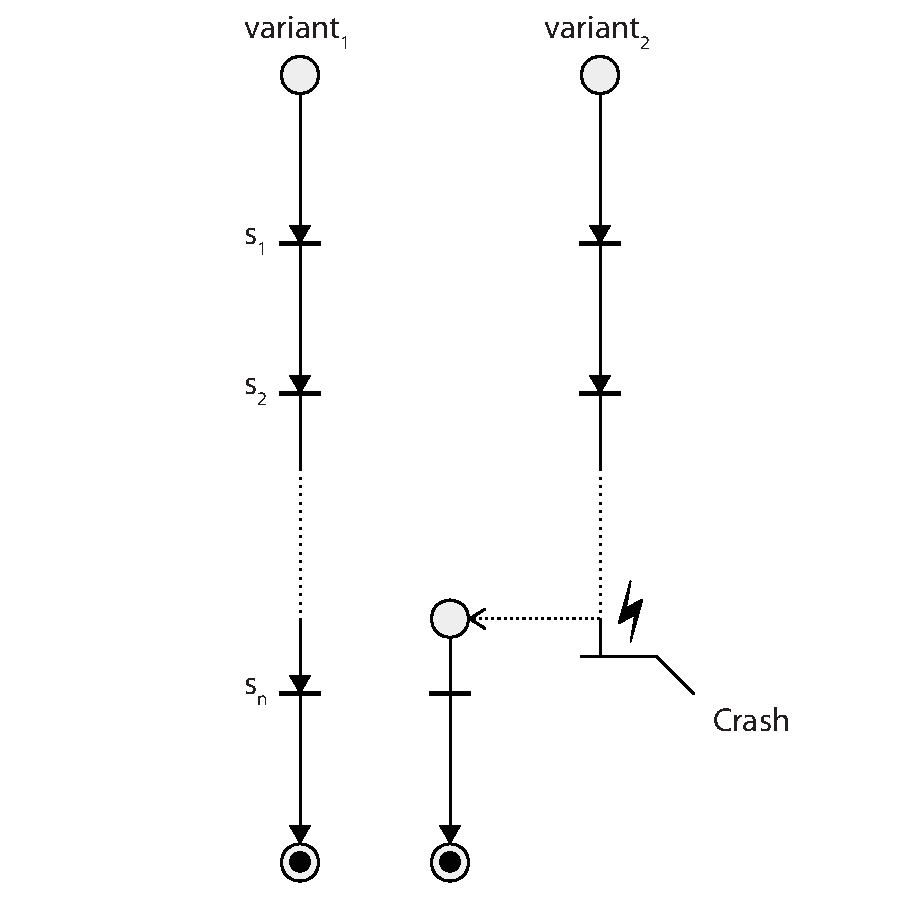
\includegraphics[width=\textwidth]{overview/figures/failrecovery}
    \caption{Failure recovery scheme.}
    \label{fig:failrecovery-scheme}
  \end{subfigure}
  \caption{Two schemes of multi-version execution presented in the thesis.}
  \label{fig:mvx-schemes}
\end{figure}

In this thesis, we present two different schemes for implementing the
multi-version execution technique. The first is the failover scheme, shown in
Figure~\ref{fig:failover-scheme}, in which $N$ different versions are being run
in parallel, and if one these versions fail, we transparently switch to other
one. This scheme offers minimal performance overhead enabling the use of large
number of versions, but offers only limited guarantees in case of failure.  In
addition, we propose a failure recovery scheme, conceptually depicted in
Figure~\ref{fig:failrecovery-scheme}, which allows program to survive errors
introduced by software patches. However, as a trade-off, this scheme introduces
a larger perfomance penalty and is limited to only two versions being run in
parallel.

% To tackle the software update problem, we propose \emph{multi-version
% execution}, a novel technique, which fits within the overall theme of
% $N$-version programming~\cite{avizienis:nvp,chen1995}. The goal of this
% technique is to improve the software update process to increase software
% availability and reliability by exploiting the abundance of resources (\eg idle
% processor time) made available by modern highly parallel platforms. Whenever a
% new system update becomes available, instead of upgrading the software to the
% newest version, we run the new version in parallel with the old one; by
% carefully coordinating their executions and selecting the behaviour of the more
% reliable version when they diverge, we create a more secure and dependable
% multi-version application. As new versions arrive, we continue to execute them
% in parallel with the existing ones, until all available resources have been
% exhausted, or a user-specified threshold has been reached.  At that point, we
% can either discard the very oldest versions, or we can use more sophisticated
% replacement strategies.

The multi-version execution technique fits within the overall theme of
$N$-version programming~\cite{avizienis:nvp,chen1995}. The goal of this
technique is to improve the software update process to increase software
availability and reliability by exploiting the abundance of resources (\eg idle
processor time) made available by modern highly parallel platforms.  We believe
that multi-version execution updates is a timely solution in the context of
today's computing platforms~\cite{multiplicity}. The last decade has seen the
emergence of new hardware platforms, ranging from multi-core processors to
large-scale data centers, which provide an abundance of computational resources
and a high degree of parallelism. These platforms already benefit applications
with a great amount of inherent concurrency.  However, there has been
relatively little progress in exploiting this abundance of resources to improve
software reliability and availability, especially in the context of software
updates.

Typical data centres are designed for peak load to ensure service-level
agreements are met. Servers are rarely completely idle but they do not operate
near their maximum utilisation; most of the time, they operate at between 10\%
and 50\% of their maximum utilization levels. However, even an energy-efficient
server consumes half its full power when doing virtually no work---and for
normal servers, this ratio is much worse~\cite{barroso2007}.  Therefore,
instead of dynamically switching off unused servers which is not effective, we
aim to use the abundance of these resources (\ie processing power) to increase
software availability and reliability.

Our approach aims to improve the reliability of the software update process by
taking advantage of idle resources---such as idle cores on a CPU and idle
servers in a data center---to run multiple versions of an application in
parallel, with the goal of improving the overall reliability and security of
the software being upgraded.  Our current focus is on multi-core processors,
but we believe this solution could be adapted to work on other parallel
platforms as well.  Furthermore, this update mechanism could be extended to
work with a large number of versions running in parallel and configured to
balance conflicting requirements such as performance, reliability and energy
consumption.

There are three main challenges that we need to address to make this approach
viable. First, we need to implement mechanisms for effectively coordinating the
parallel execution of multiple program versions.  Second, when executions
diverge, we need to select the output of the more reliable one, and potentially
merge them back once executions converge again.  Finally, we need to ensure
that the overall system is able to scale up and down the number of program
versions run in parallel in order to balance conflicting requirements such as
performance, reliability, and energy consumption.

%%%%%%%%%%%%%%%%%%%%%%%%%%%%%%%%%%%%%%%%%%%%%%%%%%%%%%%%%%%%%%%%%%%%%%%%%%%%

%We aim to tackle this problem using a simple but effective approach based on
%application-level virtualization.  Whenever a new program update becomes
%available, instead of upgrading the software to the newest version, we {\it
%run the new version in parallel with the old}.  As new versions arrive, we
%continue to execute them in parallel with the existing ones, until all
%available resources have been exhausted, or a user-specified threshold has
%been reached.  At that point, we can either discard the very oldest versions,
%or we can use more sophisticated replacement strategies.  This approach can
%be extended to work with a large number of versions run in parallel, and can
%be applied to several different platforms, ranging from multicore processors
%to large-scale data centers.  

%The rest of this paper is organized as follows. Section~\ref{sec:background}
%discusses related work and  Section~\ref{sec:motivation} motivates our
%approach by using a scenarios based on Google Chrome web browser and Vim text
%editor.  Then, Section~\ref{sec:challenges} discusses the main challenges that
%we need to address to make this approach work in practice and
%Section~\ref{sec:prototype} presents a protype implementing safe updates
%in the context of multi-core processors. Finally, Section~\ref{sec:opportunities}
%describes the potential future work and Section~\ref{sec:conclusion} concludes.

%The rest of this paper is organized as follows. Section~\ref{sec:background}
%discusses related work and  Section~\ref{sec:motivation} motivates our
%approach by using a scenarios based on Google Chrome web browser and Vim text
%editor.  Then, Section~\ref{sec:challenges} discusses the main challenges that
%we need to address to make this approach work in practice and
%Section~\ref{sec:prototype} presents a protype implementing safe updates
%in the context of multi-core processors while Section~\ref{sec:evaluation}
%shows a case study for our approach. Finally, Section~\ref{sec:opportunities}
%describes future work and Section~\ref{sec:conclusion} concludes.

%% Following work presents our approach approach, its advantages and
%% disadvantages. Furthermore, it provides comparison and summarizes
%% differences from the existing solutions aiming to achieve similar
%% goals.


